\section{Optimizing of the Relaxation Factor}
\label{Sec: Optimizing Relaxation Factor}

\begin{figure}[H]
    \centering
    \begin{subfigure}[b]{0.49\linewidth}
        \centering
        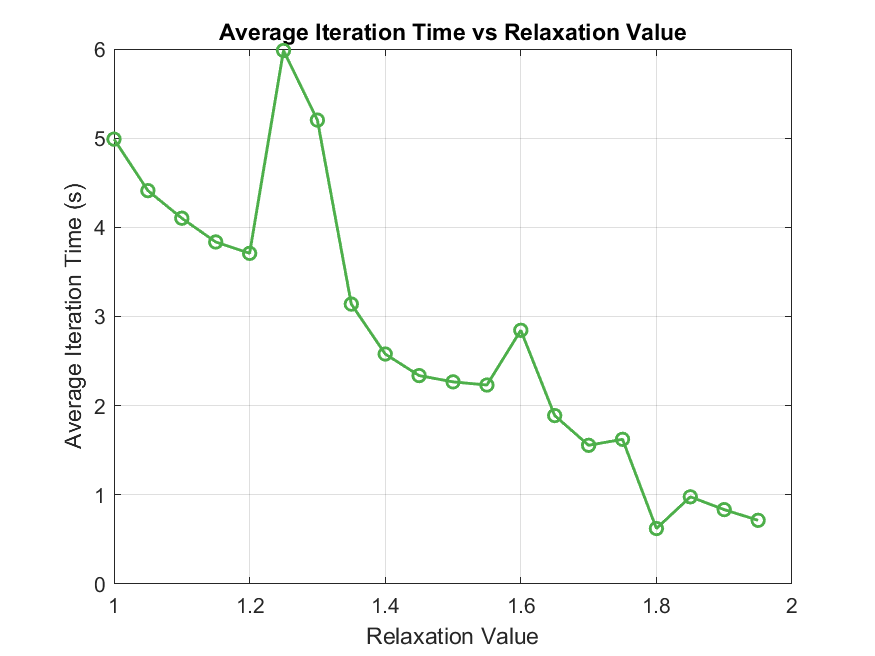
\includegraphics[width=\linewidth]{figures/overrelaxation/average_iteration_time_vs_relaxation_value.png}
        \caption{Average Iteration Time vs Relaxation Value}
        \label{fig:average_iteration_time}
    \end{subfigure}
    \hfill
    \begin{subfigure}[b]{0.49\linewidth}
        \centering
        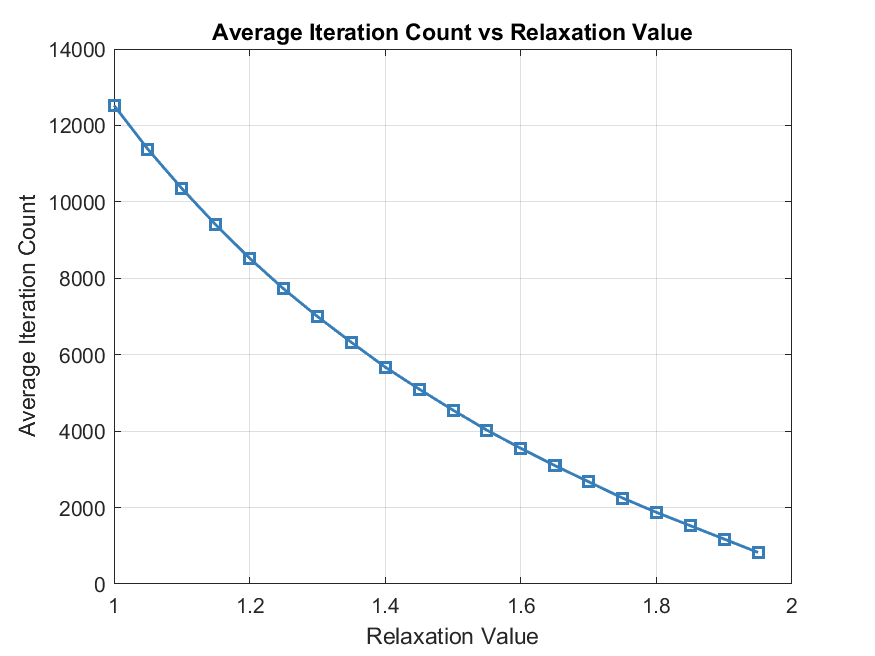
\includegraphics[width=\linewidth]{figures/overrelaxation/average_iteration_count_vs_relaxation_value.png}
        \caption{Average Iteration Count vs Relaxation Value}
        \label{fig:average_iteration_count}
    \end{subfigure}
    \caption{Comparison of Average Iteration Time and Count with Relaxation Values}
    \label{fig:comparison}
\end{figure}
